% Just The Docs Front Matter
% title: Square Ice Shelf
% parent: Tutorials
% has_children: false
% has_toc: false

\subsection{Square Ice Shelf} \label{sec:using-issm-tutorials-squareiceshelf}
This is an example of velocity computation in steady state for a square ice shelf. First, launch MATLAB. In the left sidebar, select \lstinlinebg|ISSM_DIR| (the directory in which ISSM is stored) as your Current Directory. Then, navigate to \lstinlinebg|examples/SquareIceshelf|, which you can also do via the left sidebar or by running the following in the MATLAB Command Window:
\begin{lstlisting}
>> cd examples/SquareIceShelf
\end{lstlisting}

You can create an empty model structure by running:
\begin{lstlisting}
>> md = model;
\end{lstlisting}

Create a mesh of the domain outline with a resolution of 50,000 meters:
\begin{lstlisting}
>> md = triangle(md, 'DomainOutline.exp', 50000);
\end{lstlisting}

Define the glacier system as an ice shelf (no island):
\begin{lstlisting}
>> md = setmask(md, 'all', '');
\end{lstlisting}

Parameterize the model with the file \lstinlinebg|Square.par| (which you can see exists in the current directory by inspecting the left sidebar):
\begin{lstlisting}
>> md = parameterize(md, 'Square.par');
\end{lstlisting}

Define all elements as SSA:
\begin{lstlisting}
>> md = setflowequation(md, 'SSA', 'all');
\end{lstlisting}

Compute the velocity field of the ice shelf:
\begin{lstlisting}
>> md = solve(md, 'Stressbalance');
\end{lstlisting}

Finally, generate a plot of the velocity:
\begin{lstlisting}
>> plotmodel(md, 'data', md.results.StressbalanceSolution.Vel);
\end{lstlisting}

\begin{figure}[H]
	\begin{center}
		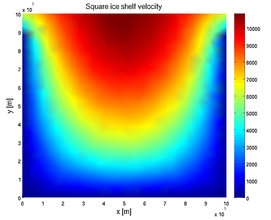
\includegraphics[width=\textwidth]{\assetsParentPath/assets/img/using-issm/tutorials/squareiceshelf/squarevel.png}
	\end{center}
\end{figure}

\clearpage % Make sure all figures are placed before next section
